\documentclass[journal]{vgtc}                % final (journal style)
%\documentclass[review,journal]{vgtc}         % review (journal style)
%\documentclass[widereview]{vgtc}             % wide-spaced review
%\documentclass[preprint,journal]{vgtc}       % preprint (journal style)
%\documentclass[electronic,journal]{vgtc}     % electronic version, journal

%% Uncomment one of the lines above depending on where your paper is
%% in the conference process. ``review'' and ``widereview'' are for review
%% submission, ``preprint'' is for pre-publication, and the final version
%% doesn't use a specific qualifier. Further, ``electronic'' includes
%% hyperreferences for more convenient online viewing.

%% Please use one of the ``review'' options in combination with the
%% assigned online id (see below) ONLY if your paper uses a double blind
%% review process. Some conferences, like IEEE Vis and InfoVis, have NOT
%% in the past.

%% Please note that the use of figures other than the optional teaser is not permitted on the first page
%% of the journal version.  Figures should begin on the second page and be
%% in CMYK or Grey scale format, otherwise, colour shifting may occur
%% during the printing process.  Papers submitted with figures other than the optional teaser on the
%% first page will be refused.

%% These three lines bring in essential packages: ``mathptmx'' for Type 1
%% typefaces, ``graphicx'' for inclusion of EPS figures. and ``times''
%% for proper handling of the times font family.

\usepackage{mathptmx}
\usepackage{graphicx}
\usepackage{times}
\usepackage{booktabs}

%% We encourage the use of mathptmx for consistent usage of times font
%% throughout the proceedings. However, if you encounter conflicts
%% with other math-related packages, you may want to disable it.

%% This turns references into clickable hyperlinks.
\usepackage[bookmarks,backref=true,linkcolor=black]{hyperref} %,colorlinks
\hypersetup{
  pdfauthor = {},
  pdftitle = {},
  pdfsubject = {},
  pdfkeywords = {},
  colorlinks=true,
  linkcolor= black,
  citecolor= black,
  pageanchor=true,
  urlcolor = black,
  plainpages = false,
  linktocpage
}

%% If you are submitting a paper to a conference for review with a double
%% blind reviewing process, please replace the value ``0'' below with your
%% OnlineID. Otherwise, you may safely leave it at ``0''.
\onlineid{0}

%% declare the category of your paper, only shown in review mode
\vgtccategory{Research}

%% allow for this line if you want the electronic option to work properly
\vgtcinsertpkg

%% In preprint mode you may define your own headline.
%\preprinttext{To appear in IEEE Transactions on Visualization and Computer Graphics.}

%% Paper title.

\title{Visualizing the TDD Cycle}

%% This is how authors are specified in the journal style

%% indicate IEEE Member or Student Member in form indicated below
\author{Michael Hilton, Mihai Codoban, and Caius Brindescu}
\authorfooter{
%% insert punctuation at end of each item
\item
 Michael Hilton is with OSU. E-mail: hiltonm@eecs.oregonstate.edu.
\item
 Mihai Codoban is with OSU. E-mail: codobanm@eecs.oregonstate.edu.
\item
 Caius Brindescu is with OSU. E-mail: brindesc@eecs.oregonstate.edu.
}

%other entries to be set up for journal
%\shortauthortitle{Biv \MakeLowercase{\textit{et al.}}: Global Illumination for Fun and Profit}
%\shortauthortitle{Firstauthor \MakeLowercase{\textit{et al.}}: Paper Title}

%% Abstract section.
%\abstract{
%} % end of abstract

%% Keywords that describe your work. Will show as 'Index Terms' in journal
%% please capitalize first letter and insert punctuation after last keyword
%\keywords{Radiosity, global illumination, constant time}

%% ACM Computing Classification System (CCS). 
%% See <http://www.acm.org/class/1998/> for details.
%% The ``\CCScat'' command takes four arguments.

%\CCScatlist{ % not used in journal version
 %\CCScat{K.6.1}{Management of Computing and Information Systems}%%
%{Project and People Management}{Life Cycle};
% \CCScat{K.7.m}{The Computing Profession}{Miscellaneous}{Ethics}
%}

%% Uncomment below to include a teaser figure.
%   \teaser{
%   \centering
%   \includegraphics[width=16cm]{CypressView}
%   \caption{In the Clouds: Vancouver from Cypress Mountain.}
%  }

%% Uncomment below to disable the manuscript note
%\renewcommand{\manuscriptnotetxt}{}

%% Copyright space is enabled by default as required by guidelines.
%% It is disabled by the 'review' option or via the following command:
% \nocopyrightspace

%%%%%%%%%%%%%%%%%%%%%%%%%%%%%%%%%%%%%%%%%%%%%%%%%%%%%%%%%%%%%%%%
%%%%%%%%%%%%%%%%%%%%%% START OF THE PAPER %%%%%%%%%%%%%%%%%%%%%%
%%%%%%%%%%%%%%%%%%%%%%%%%%%%%%%%%%%%%%%%%%%%%%%%%%%%%%%%%%%%%%%%%

\begin{document}

%% The ``\maketitle'' command must be the first command after the
%% ``\begin{document}'' command. It prepares and prints the title block.

%% the only exception to this rule is the \firstsection command
\firstsection{Introduction}

\maketitle

%% \section{Introduction} %for journal use above \firstsection{..} instead

Software processes have had little or no visualization aids.
Without this kind of information, it is hard to grasp whether these processes are followed correctly. It is hard to find anomalies, and identify potential areas for improvement. Without visualizations that show the big picture, one has to go through tedious, time consuming and incomplete data to learn how a processes was actually implemented. One has to go through reports, interviews and mine software artefacts in order to gain a big picture understanding on how a particular team implemented a software process.

We intend to build visualizations that aid in analyzing developers� TDD practice. Such visualizations would visually expose, for each developer, the main stages of the practice and how they evolve over time.

This kind of information benefits developers, managers and researchers. Developers can better improve their practice by analyzing their past behaviour. Managers can get a sense of magnitude of how well TDD is implemented in the team. Researchers can gain insights and better describe the theoretical foundations of TDD by finding patterns and exploring the divide between practical and theoretical TDD.

\section{Target Audience/User}

The target audience for this visualization is anyone who wants to know about how the software development process happened.  

Developers who want to analyze their own TDD cycle can use this visualization to examine their performance and look for ways to improve their practice.

Researchers analyzing the practice of TDD can use this to look for patterns in how TDD is actually used.  Without this visualization, the data would be a series of JSON files that would be almost impossible to get meaning from just by looking at them.  

Finally, managers analyzing the performance of those that they are managing can use this visualization to have an accurate picture of their team�s performance.

\section{High level domain question/questions of interest}

\textbf{Developers:} \\
Q1: What does my TDD workflow look like? \\
Q2: How does my TDD workflow compare to others�? \\
Q3: How does my TDD workflow change over time? \\

\textbf{Managers:} \\
Q1: How consistent are my developers in using TDD? \\
Q2: Who are the best TDD performers? \\

\textbf{Researchers:} \\
Q1: What does a practica l TDD workflow look like? \\
Q2: How does practical TDD differ from theoretical TDD? \\

\section{Detailed questions that users may ask of the data}

\textbf{Developers:} \\
Q1: What does my TDD workflow look like? 
\begin{itemize}
	\item What part of the TDD cycle to I spend the most time in?
	\item What part of the TDD cycle do I write the most code in?
	\item How close does my workflow compare with ideal TDD?
	\item What code did I write for a specific TDD stage?
\end{itemize}

Q2: How does my TDD workflow compare to others�?
\begin{itemize}
	\item How does the time I spend in each TDD cycle compare to others?
	\item How does the code I write in each TDD cycle compare to others?
	\item How close is my workflow to the ideal TDD in comparison with others?
\end{itemize}

Q3: How does my TDD workflow change over time?
\begin{itemize}
	\item Is my TDD workflow consistent?
	\item How does the time I spend in each TDD cycle change over time?
	\item How does the amount of code I write in each TDD cycle change over time?
\end{itemize}

\noindent\textbf{Managers:} \\
Q1: How consistent are my developers in using TDD?
\begin{itemize}
	\item How much time does each developer spend in each TDD cycle?
	\item How much code does each developer write in each TDD cycle?
	\item How much time do all developers spend in each TDD cycle on average?
	\item How much code do all developers write in each TDD cycle on average?
	\item What percentage of the code my developers write conforms to the TDD model?
\end{itemize}

Q2: Who are the best TDD performers? 
\begin{itemize}
	\item Which developers have a process that is closest to the ideal TDD process?
	\item Which developers spend the least/most time in each TDD cycle?
	\item Which developers write the least/most code in each TDD cycle?
\end{itemize}
	
\noindent\textbf{Researchers:}
Q1: What does a practical TDD workflow look like?
\begin{itemize}
	\item How much time do TDD developers spend in each TDD cycle?
	\item How much code do TDD developers write in each TDD cycle?
	\item What percentage of code that developers write follows the ideal TDD model?
\end{itemize}
	
Q2: How does practical TDD differ from theoretical TDD?
\begin{itemize}
	\item What are patterns that we can identify in how developers write using the TDD process?
	\item How does the time TDD developers spend in each cycle compare with our reference implementation of the TDD process?
	\item How does the code TDD developers write in each cycle compare with our reference implementation of the TDD process?
\end{itemize}

\section{Abstract operations/tasks that must be supported in order to answer the detailed questions
}

Compute TDD cycles: starting from low level text edits, cluster the edits according to the TDD cycle stages: red, green, blue. \\
 
\noindent\textbf{DQ1a:} Compute TDD cycles. Compare cycle stage times \\
\textbf{DQ1b:} Compute TDD cycles. Compare cycle stage size \\
\textbf{DQ1c:} Compute TDD cycles. Retrieve ideal TDD cycles. Compare user cycles and style with theoretic TDD variants \\
\textbf{DQ1d:} Compute TDD cycles. Retrieve code edits for specific cycle  or stage. \\
 
\noindent\textbf{DQ2a:} Compute TDD cycles. Retrieve cycles for specific developers. Compare developer cycle times with other cycles. \\
\textbf{DQ2b:} Compute TDD cycles. Retrieve cycles for specific developers. Compare developer cycle size with other cycles. \\
\textbf{DQ2c:} Compute TDD cycles. Retrieve cycles for specific developers. Retrieve ideal TDD cycles. Compare developer and others against ideal TDD cycle. \\
 
\noindent\textbf{DQ3a:} Compute TDD cycles. Derive variance of TDD cycle metrics. Characterize distribution of variance \\
\textbf{DQ3b:} Compute TDD cycles. Derive variance of TDD cycle times. Characterize distribution of time variance \\
\textbf{DQ3c:} Compute TDD cycles. Derive variance of TDD cycle sizes. Characterize distribution of cycle size variance \\
 
\noindent\textbf{MQ1a:} Compute TDD cycles. Retrieve cycles for specific developers. Characterize distribution of cycle times. Compare distributions between developers. \\
\textbf{MQ1b:} Compute TDD cycles. Retrieve cycles for specific developers. Characterize distribution of cycle size. Compare distributions between developers. \\
\textbf{MQ1c:} Compute TDD cycles. Retrieve cycles for specific developers. Derive average TDD cycle times of developers. \\
\textbf{MQ1d:} Compute TDD cycles. Retrieve cycles for specific developers. Derive average TDD cycle size of developers. \\
\textbf{MQ1e:} Compute TDD cycles. Retrieve cycles for specific developers. Retrieve ideal TDD cycles. Compare with ideal TDD \\
 
\noindent\textbf{MQ2a:} Compute TDD cycles. Retrieve cycles for specific developers. Retrieve ideal TDD cycles. Compare with ideal TDD. Derive developer closest to ideal TDD \\
\textbf{MQ2b:} Compute TDD cycles. Retrieve cycles for specific developers. Retrieve ideal TDD cycles. Retrieve cycle times. Compare with ideal TDD. Find range of developers with times closest and farthest away from ideal TDD. \\
\textbf{MQ2c:} Compute TDD cycles. Retrieve cycles for specific developers. Retrieve ideal TDD cycles. Retrieve cycle sizes. Compare with ideal TDD. Find range of developers with cycle sizes closest and farthest away from ideal TDD. \\
 
\noindent\textbf{RQ1a:} Compute TDD cycles. Retrieve cycles for specific developers. Derive average TDD cycle times of developers. \\
\textbf{RQ1b:} Compute TDD cycles. Retrieve cycles for specific developers. Derive average TDD cycle size of developers. \\
\textbf{RQ1c:} Compute TDD cycles. Retrieve cycles for specific developers. Retrieve ideal TDD cycles. Compare with ideal TDD \\
 
\noindent\textbf{RQ2a:} Compute TDD cycles. Retrieve cycles for all developers. Find clusters of similar cycles. Derive periodicity of clusters. \\
\textbf{RQ2b:} Compute TDD cycles. Retrieve cycles for all developers. Retrieve ideal TDD cycles. Retrieve cycle times. Compare with ideal TDD. \\
\textbf{RQ2c:} Compute TDD cycles. Retrieve cycles for all developers. Retrieve ideal TDD cycles. Retrieve cycle sizes. Compare with ideal TDD. \\

\section{Data type abstractions}

\begin{table}[hbt]
\begin{tabular}{l l l}
\toprule
Variable & Type & Expected value \\
\midrule
Event type & Nominal & textChange, testRun, etc \\
Event timestamp & Quantitative & UNIX timestamp \\
Event Source & Nominal & user, cut/copy/paste, etc \\
Text Added & Nominal & string \\
Offset & Quantitative & location from file start \\
Length & Quantitative & size of text edit \\
File Changed & Nominal & The path of the file being changed \\
Test Outcome & Nominal & Pass/Fail/Error \\
Test Duration & Quantitative & Number of seconds the test took \\
Launch & Nominal & Application start and stop \\
Refactoring type & Nominal & Refactorings done \\
\bottomrule
\end{tabular}
\end{table}

Data is gathered by a plugin that is installed by the user in her IDE. The plugin records all the events from the event table and sends them to a server.

\section{Encodings}

\subsection{Overview}

For this design iteration we only focus on the single developer scenario. Thus we do not tackle design solutions for user questions that involve managers or researchers.

Our single user solution proposes the visualization of data at several abstraction levels, as \cite{two} suggests. Thus users have three scopes at which they can analyze their TDD practice, varying from concrete to abstract:

\textbf{Text change level.} The user can browse through individual text changes to see how they relate to TDD stages. We call this visualization the �TDD Atomic Chart�

\textbf{TDD cycle stage level.} The user can browse through the stages of their TDD cycles. We call this visualization the �TDD Spectrum Chart� and is inspired by \cite{one}.

\textbf{TDD cycle level.} The user can browse through high level TDD cycles. We call this visualization the �TDD Sun Chart� and is reminiscent of radar charts.

Figure~\ref{fig:one} shows a sketch of the single developer TDD workbench.
The top bar contains the high level, abstract visualizations of the TDD cycles. The upper part represents the TDD Spectrum Chart while the bottom part represents the TDD Sun Chart. 

\begin{figure*}[hbt]
	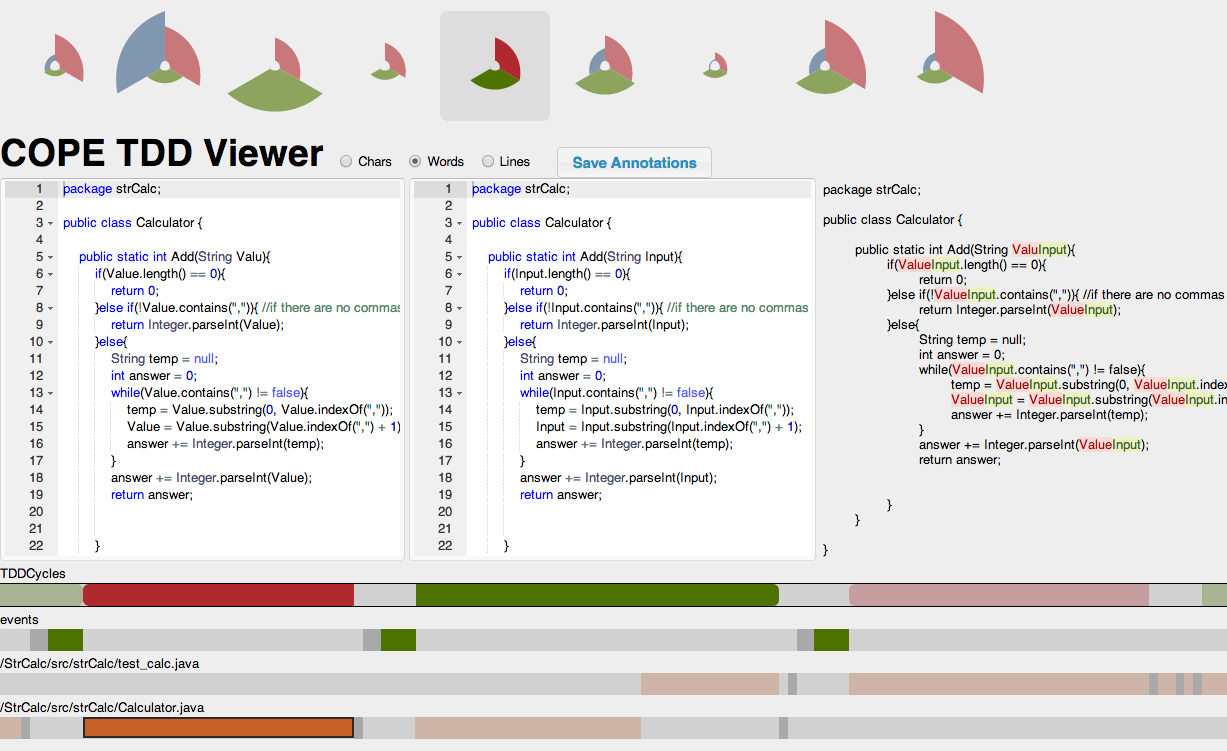
\includegraphics[width=\textwidth]{fig1}
	\caption{Overall view}
\label{fig:one}
\end{figure*}

The bottom bar shows the TDD Atomic chart. It is mainly a change navigation tool that users use to browse through granular code changes. The mapping from code changes to TDD stages is present via the top band.

In the middle there are three editors that show the code changes between two arbitrary points in the TDD Atomic Chart. The first two editors show the first and the last variant of the code while the third shows the diff between the two: green highlights for added text and red highlight for deleted text.

\section{TDD Atomic Chart}

\subsection{Justification}

This visualization allows the developer to navigate through the code events.
Each coding event is abstracted away via a rectangle. Moreover, the events are grouped by the files in which they are performed. The event rectangles are sorted via their timestamps. Temporal data abstraction and data clustering techniques from \cite{one} inspired this visualization: complex coding events are abstracted via rectangles and event types are clustered: event types are encoded via square color. A similar visualization is the Cluster Calendar View presented in \cite{one}.

The temporal succession of rectangles also provides the affordance of time flow. It resembles soundwave amplitude visualization from sound editors and music players.
However, one key difference from a sound editor is that while the sound editor shows continuous data, we show cycle snapshots, so our visualization resembles more closely small multiples.

Since developers� main concern with the tool is the study of TDD, we provide a mapping to TDD cycles at text change level as well thus presenting TDD relevant data at various abstraction levels. Since TDD stages are aligned with coding events, the users would tend to instinctively visually group code changes by TDD stage (gestalt principle: instinctively continuing an interrupted interval).
The TDD stages are differentiated by their color. TDD literature uses red, green and blue to differentiate various stages.

Encoding (using Mackinlay�s Ranking):
\begin{enumerate}
	\item Temporal succession of coding events (qualitative): position
	\item Temporal succession of TDD stages (qualitative): position. Since coding events and TDD stages are on separate axis, both can use the position encoding.
	\item Event type (qualitative): color
	\item TDD stage (qualitative): color. Since coding events and TDD stages are on separate axis, both can use the position encoding.
\end{enumerate}

\section{TDD Spectrum Chart}

\subsection{Justification}

The visualization in Figure~\ref{fig:two} enables developers, managers and researchers to answer many of their questions. It shows the succession of TDD cycle stages in time. Each TDD stage appears as a rectangle. We chose rectangles because we can encode two TDD metrics with it: cycle code change size and cycle duration.

\begin{figure*}
	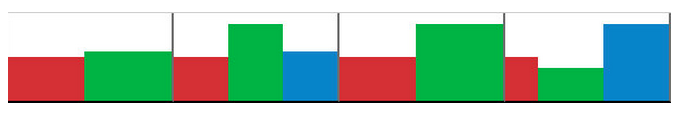
\includegraphics[width=\textwidth]{fig2.png}
	\caption{TDD Spectrum Chart}
	\label{fig:two}
\end{figure*}

We ordered our encodings using Mackinlay�s ranking.
Since the TDD cycle is defined by a temporal repetition of stages, the sequence of stages (categorical data) is encoded via position on the Ox axis.
TDD stage size metrics are encoded using the rectangle width (time) and height (amount of code). Position being taken, they take the second encoding for quantitative data, length.
The TDD stage type (categorical) is encoded via color: red for tests, green for development and blue for refactoring. Color occupies the second ranking for categorical data.

With this information the users can answer questions about what part of the TDD cycle they spend the most time on and how big their cycles are. They can also analyze how their cycles vary over time and whether any patterns occur.

Moreover, users can compare the TDD cycles for several users by showing several TDD time series side by side. This allows comparison of how much time different developers spend in stages, how big their stages are and whether they follow TDD at all.

\section{TDD Sun Chart}

\subsection{Justification}

The purpose of this visualization is to represent an entire TDD cycle by just one shape. 
See figure~\ref{fig:three}
By doing so, users obtain a singular mental image of an entire TDD cycle.
\cite{one} presents this technique as temporal data abstraction, in which complex, large temporal data is abstracted and mapped to qualitative entities, in our case, shape.

\begin{figure*}
	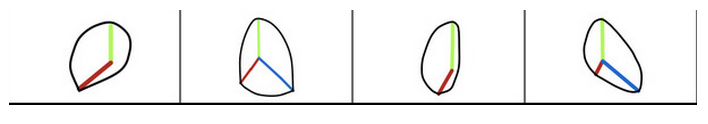
\includegraphics[width=\textwidth]{fig3.png}
	\caption{TDD Sun Chart}
	\label{fig:three}
\end{figure*}

The visualization is based on a radar chart with three axis. The axis represent the size of each of three TDD cycle stages. These three axis generate the shape of a particular TDD cycle.

Instead of using straight lines to connect the radar chart points, we use curved lines. Together they create a deformed circle. Thus the unique size characteristics of each TDD cycle are encoded into the deformation of the circle. We used a circle and not a square due to gestalt principles: the vertices of the square introduce discontinuity in perception, and biases the viewer to the number 4. A circle on the hand has no vertices (points of discontinuity) and therefore does not introduce deformation bias. Thus, we hypothesize that circles show deformation in a more unbiased way than squares.

As with the timeseries chart, the sequence of TDD eggs are encoded via position, due to the temporal cyclic property of TDD cycles. We thus obtain small multiples snapshots of how the TDD cycle progresses in time.
TDD cycle metrics are encoded via the next available encoding, length (the radar chart axis).

Encoding (using Mackinlay�s Ranking):
\begin{enumerate}
	\item Succession of TDD stages (quantitative): position
	\item TDD stage size metrics (quantitative): length
\end{enumerate}
 
%% if specified like this the section will be committed in review mode
%\acknowledgments{}

\bibliographystyle{abbrv}
%%use following if all content of bibtex file should be shown
%\nocite{*}
\bibliography{design-pass-1}
\end{document}

